% !TeX document-id = {5f9589b8-498a-4233-98c1-605de3ca7afa}
% !TeX TXS-program:compile = txs:///pdflatex/[--shell-escape]


\documentclass[12pt, paper=a4, bibtotoc, toc=listof, headsepline=true]{scrreprt}

\usepackage[a4paper, includeheadfoot, %bindingoffset=3cm, 
left=2.7cm, right=2.7cm, top=2.5cm, bottom=3cm]{geometry}

%Header
\usepackage[automark]{scrpage2}
\pagestyle{scrheadings}
\clearscrheadfoot
\ohead{\rightmark}
\cfoot[\pagemark]{\pagemark}
\renewcommand*{\chaptermarkformat}{}
\renewcommand*{\headfont}{\normalfont}


%\setlength{\headheight}{12mm} % Höhe der Kopfzeile 




\setheadsepline[text]{0.4pt} % Trennlinie unter Kopfzeile 
%Abstand nach Header Trennlinie
%\usepackage[headsep=5mm]{geometry}

%\setfootsepline[text]{0.4pt} % Trennlinie unter Fußzeile






\setcounter{tocdepth}{3}% Include \subsubsection in ToC
\setcounter{secnumdepth}{3}% Number \subsubsection
\setuptoc{toc}{numbered} % Adds ToC to ToC toDo: remove Pagenumber of ToC in ToC

\usepackage[ngerman]{babel} %Deutsch

\usepackage[utf8]{inputenc} %UTF8 Formatierung

\usepackage[T1]{fontenc}

\usepackage{helvet} %Arial
\renewcommand{\familydefault}{\sfdefault} %Arial

\usepackage{float}
\newfloat{listing}{tbhp}{lst}%[section]
\floatname{listing}{Listing}
\newcommand{\listoflistings}{\listof{listing}{Listing Verzeichnis}}

\usepackage{chngcntr}% http://ctan.org/pkg/chngcntr
\counterwithin{listing}{chapter} %counts chapters of listing




\usepackage[chapter]{minted} %Code Formatierung
\newminted{JavaScript}{frame=single,framesep=10pt, linenos, breaklines=true}
\newminted{HTML}{frame=single,framesep=10pt, linenos, breaklines=true}

\usepackage{caption}
\DeclareCaptionFont{black}{\footnotesize\color{black}}
\DeclareCaptionFormat{listing}{{\parbox{\linewidth-2\fboxsep}{#1#2#3}}}
\setkomafont{captionlabel}{\usekomafont{caption}}




%Caption Listing, Figure Styling
\captionsetup[listing]{labelfont=black,textfont=black} %Caption of Listing
\captionsetup[figure]{labelfont=black,textfont=black} %Caption of Figure

\usepackage{graphicx} %IMG

\usepackage{csquotes}

\usepackage[onehalfspacing]{setspace} %Zeilenabstand


\usepackage[
	backend=biber,
	style=numeric,
	sorting=none
	]{biblatex}
\addbibresource{library.bib}

\usepackage{acronym}

% Neues cite-Kommando oder altes \footcite-Kommando überschreiben
\DeclareCiteCommand{\smfootcite}[\mkbibfootnote]
{\usebibmacro{prenote}}                                 
{\usebibmacro{citeindex}%
	\setunit{\addnbspace}
	\printnames{labelname}%
	\setunit{\labelnamepunct}
	\newunit
	\printfield{year}
}
{\addsemicolon\space}
{\usebibmacro{postnote}}


\renewcommand{\smfootcite}[2][2]{\relax}





\title{Erstellung von adaptiven Web Components}
\author{Christoph Kleber}
\date{\today}

\begin{document}
\maketitle

\chapter*{Kurzfassung}
\addcontentsline{toc}{chapter}{Kurzfassung}
In dieser Arbeit geht es um Web Components.
	
\chapter*{Abstract}
\addcontentsline{toc}{chapter}{Abstract}
This thesis is about Web Components.

\listoflistings
\listoffigures

\chapter*{Abkürzungsverzeichnis}
\addcontentsline{toc}{chapter}{Abkürzungsverzeichnis}
\begin{acronym}
	\acro{API}{Advanced Programming Interface}
	\acro{DOM}[DOM]{Document Object Model}
	\acro{HTML}[HTML]{Hypertext Markup Language}
	\acro{URL}[URL]{Uniform Resource Locator}
	\acro{HTML5}[HTML5]{Hypertext Markup Language Version 5}
	\acro{CSS}[CSS]{Cascading Style Sheets}
	\acro{W3C}{World Wide Web Consortium}
	\acro{REST}{Representational State Transfer}
	\acro{HTTP}{Hypertext Transfer Protocol}
	\acro{JSON}{JavaScript Object Notation}
	\acro{WCAG 2.0}{Web Content Accessibility Guidelines 2.0}
\end{acronym}

\tableofcontents

\chapter{Adaptivität}
	\section{Begriffsklärung}
	Der Begriff Adaptivität wird in vielen verschiedenen Kontexten genutzt. Die Bedeutung ist somit mehrdeutig und abhängig vom Umfeld. Beispielsweise wird in der Psychotherapie unter Adaptivität im therapeutischen Vorgehen eine \enquote{Grundhaltung [beschrieben], welche die Bereitschaft impliziert, unter stetiger Reflexion der Prozesse von Übertragung und Gegenübertragung flexibel auf die jeweils aktuellen Bedürfnisse des Patienten einzugehen}\cite[S. 45]{woeller2014tiefenpsychologisch} Im Kontext von Datenbanken und der \enquote{Adaptivität an unterschiedliche Anforderungen} wird von Verfahren gesprochen, die \enquote{die Anpassungsfähigkeit an unterschiedliche Anforderungen und damit auch an verschiedene Einsatzumgebungen [erhöhen].}\cite[][S. 112]{loeser2013web}
	In der Softwareentwicklung kann Adaptivität folgendermaßen beschrieben werden.\enquote{Interaktive Softwaresysteme werden von Benutzern mit unterschiedlichsten Zielen, Interessen, Fähigkeiten, Erfahrenheitsgraden und Präferenzen verwendet. Um einem möglichst breiten Personenkreis zugänglich zu sein, bieten viele derzeit erhältliche Programme bereits die Möglichkeit, daß Benutzer (oder Systemadministratoren) in bestimmtem Ausmaß eine Anpassung des Programms an die jeweiligen individuellen Präferenzen vornehmen können.}\cite[S. 1]{Kobsa1993}
	\newline In den verschiedenen Auslegungen des Wortes ist ein Muster zu erkennen. Adaptivität kann definiert werden als die Fähigkeit eines Objekts, dies kann beispielsweise eine Person oder ein System sein, sich an seine Umgebung anzupassen. Diese Anpassung basiert auf bestimmten Einflüssen, so kann sich eine Datenbank an äußere Einflüsse, wie beispielsweise ihre Einsatzumgebung anpassen oder ein Softwaresystem an die Vorlieben seines Nutzers anpassen. Dies kann automatisch geschehen. So passt sich beispielsweise der Inhalt der Seite \enquote{Facebook} aufgrund eines Algorithmus an den einzelnen Nutzer an, ohne dass dieser bestimmte Einstellungen vornehmen muss.\cite[vgl.]{Rixecker2016} Die Möglichkeit zur Adaptivität kann jedoch auch dem Nutzer bereitgestellt werden. Ist dies der Fall, kann der Nutzer beispielsweise die Benutzeroberfläche an seine eigenen Vorlieben anpassen. So kann zum Beispiel die Benutzeroberfläche der Entwicklungsumgebung \enquote{JetBrains PhpStorm} anhand persönlicher Präferenzen angepasst werden und Farbstile und Kontraste angepasst werden.
	\newline
	Hier stellt sich jedoch die Frage, wie im Zusammenhang von Internetanwendungen eine Adaptivität bereitgestellt werden kann und insbesondere, an welche Aspekte sie sich anpassen soll. Hierfür muss die Umgebung, der Nutzer und auch dessen Arbeitsaufgaben erforscht und definiert werden.
	\section{Nutzungskontext}
	Die Betrachtung des Nutzungskontext bietet diese Möglichkeit. Der Nutzungskontext wird nach der DIN EN ISO 9241-210 von den Benutzermerkmalen, Arbeitsaufgaben und der organisatorischen, technischen und physischen Umgebung bestimmt. Im folgenden wird ein Überblick dieser Beschreibung gegeben.
	\begin{description}  
		\item  [Nutzer und sonstige Interessengruppen] 
		Zu Beginn sollten die Nutzergruppen und weitere Interessengruppen identifiziert und deren wesentliche Ziele und Einschränkungen beschrieben werden.
			
		\item [Merkmale der Nutzer oder Nutzergruppen]
		Diese Merkmale können \enquote{Kenntnisse, Fertigkeiten, Erfahrung, Ausbildung, Übung, physische Merkmale, Gewohnheiten, Vorlieben und Fähigkeiten einschließen.}\cite[S.16 ]{hoffmann2014venus} Sie beschreiben also insgesamt den Nutzer, um diesen besser einordnen und sich besser an diesen anpassen zu können.
		
		\item  [Ziele und Arbeitsaufgaben der Nutzer]
		Auf der einen Seite sollten die Ziele der Nutzer beschrieben werden, auf der anderen Seite die Gesamtziele des Systems. Danach sollten die Arbeitsaufgaben betrachtet und nach ihren Merkmalen untersucht werden, beispielsweise wie oft eine Aufgabe ausgeführt werden soll.
			
		\item [Umgebung(en) des Systems]
		Die Umgebung lässt sich in die technische Umgebung, also die der Computerkomponenten und Anwendungen, die physikalische Umgebung, also Aspekte wie beispielsweise Beleuchtung und soziale und kulturelle Umgebung aufteilen.Zur kulturellen Umgebung zählen beispielsweise die Arbeitsweise und Einstellungen der Umgebung des Systems.\cite[vgl. S.15 ff.]{hoffmann2014venus}
	\end{description}
	Insgesamt lässt sich somit sagen, dass die Adaptivität an den Nutzungskontext ausgerichtet werden kann. Verschiedene Merkmale des Nutzungskontext haben Einfluss darauf, wie die Adaptivität, passend zur Situation, erfolgen sollte.
		
\chapter{Web Components}
	\emph{Web Components} sind eine \ac{W3C} Spezifikation. Diese soll es ermöglichen, eigenständige und wiederverwertbare Komponenten für Web Anwendungen zu erstellen. \cite[vgl. S. 1]{patel2015learning} Sie setzen sich zusammen aus den vier Technologien \emph{Custom Elements}, \emph{\ac{HTML} Imports}, \emph{Templates} und \emph{Shadow \ac{DOM}}. Das Nutzen dieser Technologie soll Applikationen im Web leichter wiederverwertbar, wartbar, unabhängiger und kapselbar machen.\cite[vgl. S.2]{patel2015learning}
	\section{Geschichte der Web Components}
	\label{ref:gesVonWebCom}
	\emph{Web Components} wurden vom \ac{W3C} das erste Mal im Jahr 2012 als ein \emph{Working Draft}, also Arbeitsentwurf, erwähnt. Hier wurde es auch \emph{Component model for the web} genannt und bestand aus den vier Technologien \emph{Templates}, \emph{Decorators}, \emph{Custom Elements} und \emph{Shadow DOM}. In der derzeitigen Version der \emph{Web Components} wird die \emph{Decorators} Technologie nicht mehr verwendet. Die \emph{\ac{HTML} Import} Technologie wurde jedoch zu den \emph{Web Components} ergänzt.\cite[vgl.]{Cooney2012} Da die \emph{Web Components} aus verschiedenen Technologien zusammengesetzt sind, wird in dem nächsten Abschnitt auf die Geschichte der einzelnen Technologien eingegangen, um einen Überblick zu verschaffen. Hierbei wird insbesondere auf die erste Unterstützung der Technologien in den verschiedenen Browsern und die heutige Browserkompatibilität eingegangen.
		\subsection{Custom Elements !v0 und v1!}
		\emph{Custom Elements} liegen in der Version v0 und in der Version v1 vor. Die Version v0 wurde das erste Mal im Jahr 2014 von den Browsern \emph{Chrome} in der Version 33 und \emph{Opera} in der Version 20 unterstützt. In den mobilen Varianten dieser Browser  wird sie seit 2016 von \emph{Opera for Android} in der Version 37 und von \emph{Chrome for Android} in der Version 53 unterstützt.\cite[vgl.]{C2015} Im \emph{Android} Browser wird diese Version schon seit 2014 unterstützt, in der \emph{Android} Version 4.4.4. Im \emph{Samsung Internet} wird sie seit 2016 in der Version 4 genutzt.\cite[vgl.]{cusEleCanIUse} Die Version v0 wird von der Version v1 abgelöst, hier ergeben sich einige Änderungen in der Syntax der \ac{API}.\cite[vgl.]{Bidelman2016cusElev1} Derzeit wird sie nicht per Standardeinstellung von anderen Browsern unterstützt.\cite[vgl.]{firefox} Die Version v1 wird derzeit nur von den Browsern \emph{Chrome} und \emph{Opera} unterstützt. Das erste mal wurde sie im Jahr 2016 in der \emph{Chrome} Version 54 und in der \emph{Opera} Version 41 genutzt. \cite[vgl.]{C2016}
		\subsection{HTML Imports}
		\emph{\ac{HTML} Imports} wurden in den Browsern \emph{Chrome} und \emph{Opera} zuerst 2014 unterstützt. Die \emph{Imports} wurden als Erstes in der \emph{Chrome} Version 36 und in der \emph{Opera} Version 23 genutzt. Gegenwärtig wird die Technologie von den zuvor erwähnten Browsern auch in den mobilen Browser-Varianten unterstützt, in den Versionen 53 des \emph{Chromium} und 37 des \emph{Opera for Android}.\cite[vgl.]{Morrita2015} Der \emph{Android} Browser unterstützt \emph{\ac{HTML} Imports} seit 2016 in der Version 53. Der Browser des \emph{Android} Betriebssystems ist ab dem Jahr 2016 in der Version 53 kongruent mit dem Chromium Browser. \emph{Samsung Internet} unterstützt die \emph{Imports} seit 2016 in der Version 4.\cite[vgl.]{htmlTemplCaniuse}
		\subsection{Decorators}
		\emph{Decorators} erscheinen nur in Dokumenten und Artikeln, sie wurden nie von Browsern implementiert. So wird im Jahr 2012 in einem \emph{Working Draft} des \ac{W3C} von einem Beispiel gesprochen: \enquote{Here is an example of how decorators could be used to implement a simple variant of the details element}.\cite{Cooney2012} Dies zeigt, dass an dieser Stelle noch keine Implementierung dieser Technologie vorliegt. Auch in einem Arbeitsentwurf des \ac{W3C} vom Jahr 2013 wird davon gesprochen, dass \enquote{Decorators, unlike other parts of Web Components, do not have a specification yet.}\smfootcite[][]{Cooney2013}
		Auf einer aktuellen Übersichtsseite des Konsortiums wird die \emph{Decorators} Technologie nicht mehr im Zusammenhang mit \emph{Web Components} erwähnt.\cite[vgl.]{WebComCur2016}
		\subsection{Templates}
		\emph{Templates} werden schon über einen längeren Zeitraum in den verschiedenen Browsern unterstützt. Zuallererst wurden sie im \emph{Chrome} im Jahr 2013 verwendet, in der Version 26. Im selben Jahr wurden sie vom \emph{Firefox} Browser in der Version 22 und vom \emph{Opera} Browser in der Version 15 unterstützt.\cite[vgl.]{W2015}\cite[vgl.]{htmlTemFire}
		Im Jahr 2015 wurden sie dann vom \emph{Edge} Browser unterstützt, in der Version 13.\cite[vgl.]{build10547}
		Auf den Browsern des \emph{Macintosh} Betriebssystems wurden \emph{Templates} zuerst 2014 verwendet, in der \emph{Safari} Version 7.1 und der \emph{Safari \& Chrome for iOS} Version 8.\cite[vgl.]{htmlTemplCaniuse} In den meisten mobilen Varianten der Browser werden \emph{Templates} seit 2016 bereitgestellt. So erschien diese Funktion in dem \emph{Opera for Android} Browser in der Version 37, in \emph{Chrome for Android} in 53, in \emph{Firefox for Android} in 49 und im \emph{Samsung Internet} Browser in der Version 4. Der Standard Android Browser unterstützt \emph{Templates} jedoch schon seit 2013, in der Version 4.4\cite[vgl.]{htmlTemplCaniuse}
		\subsection{Shadow DOM}
		Der \emph{Shadow \ac{DOM}} existiert in der Version v0 und in der Version v1. Die Version v0 wird seit 2014 vom \emph{Chrome} in der Version 35 und \emph{Opera} Browser in der Version 21 unterstützt. Mit der Safari Version 10 kann der \emph{Shadom \ac{DOM}} seit 2016  genutzt werden.\cite[vgl.]{NiwaShaDom} Die mobilen Varianten der Browser unterstützen das \emph{Shadow \ac{DOM}} seit 2016, \emph{Opera} in der Version 37 und \emph{Chrome} in der Version 53, somit auch der \emph{Android} Browser.\cite[vgl.]{Hayato2016} Die Version v0 wird von der Version v1 abgelöst, welche verschiedene Neuerungen in der Syntax, aber auch in der Unterstützung von bestimmten Funktionen aufweist. So kann beispielsweise in der v0 ein \emph{shadow root} immer nur als \enquote{open} definiert werden, in der v1 kann er auch als \enquote{closed} \emph{shadow root} erstellt werden.\cite[vgl.]{Ito2016}
		Die Version v1 wird noch nicht in so großem Ausmaß wie die Version v0 unterstützt. Vollständig wird sie nur vom \emph{Chrome} 53 und \emph{Opera} 40 Browser unterstützt, jeweils seit 2016. In den mobilen Versionen wird sie nur von dem \emph{Chromium} und somit auch auf \emph{Android} in der Version 53 unterstützt.\cite[vlg.]{Hayato2016a}
	\section{Vergleich Webentwicklung mit Web Components und ohne}
	Das \emph{Frontend} von modernen Webseiten basiert heutzutage hauptsächlich auf den Technologien \ac{HTML}, \ac{CSS} und JavaScript. Meistens werden darüber hinaus noch verschiedene \emph{Frameworks} verwendet. \enquote{A computer system framework has a layered structure that can incorporate servers, operating systems, client machines, and applications. The framework can provide a set of functions to definde application interfaces, the interrelationships between applications, and internal communications between clients and external to online platforms}.\cite[S.15]{stuart2013roadmap} Ein \emph{Framework} ist somit ein System, das den Entwicklern bestimmte Funktionalitäten zur Verfügung stellt, ohne dass dieser sie selbst programmieren muss. Diese können beispielsweise die Hilfe bei der Interaktion mit dem \ac{DOM} sein, wie das JavaScript \emph{Framework} \enquote{jQuery}, ein \enquote{Slide-Element} bereitstellen wie das \emph{Framework} \enquote{Slider} oder zur Diagrammerstellung genutzt werden wie das \emph{Framework} \enquote{D3}. Hier ergibt sich ein Problem. Wenn in einer Applikation mehrere \emph{Frameworks} und Technologien für verschiedene Funktionen verwendet werden, können diese sich gegenseitig beeinflussen. So können die Stil-Regeln verschiedener Teile der Webseite sich unbeabsichtigt beeinflussen oder das JavaScript, welches eine bestimmte Funktion hat, an einer anderen Stelle für welche es nicht programmiert wurde, Einfluss nehmen. Darüber hinaus können viele Teile der Webseite weder wiederverwendet, noch gut gewartet werden, da sie großen Einfluss aufeinander nehmen und somit sehr ineinander verschachtelt sind.
	Die \emph{Web Components} versuchen diese Probleme durch eine (in Zukunft) native Implementierung verschiedener Techniken anzugehen, welche eine Kapselung, eine Wiederverwendung und eine leichtere Wartbarkeit von Programmcode ermöglichen sollen.			
		\subsection{Vorteil: Wenn Browserunterstützung gegeben: native, kein Framework}
		Aufgrund der Erkenntnisse der Geschichte von \emph{Web Components} in Kapitel \ref{ref:gesVonWebCom} ist eine große Wahrscheinlichkeit gegeben, dass die Technologien der \emph{Web Components} in Zukunft nativ von den verschiedenen Browsern unterstützt werden.
		Sollte dieser Fall eintreffen ergibt sich daraus ein großer Vorteil. Es muss bei der Nutzung nativer, also von den Browsern implementierten Techniken, kein externer Programmcode genutzt werden um bestimmte Funktionen abzudecken. Viele Funktionalitäten können einfach über die Nutzung nativer Methoden abgebildet werden. Deshalb müssen weniger Funktionen selbst geschrieben werden und weniger, beziehungsweise unter Umständen keine \emph{Frameworks} genutzt werden. Dies verkleinert das Laden von externen Programmcode. Darüber hinaus ist die Syntax und Funktionsweise bei nativen Funktionen bekannt und eindeutig. Daraus ergeben sich weniger Inkonsistenzen in der Programmierung und eine leichtere Verständlichkeit. Im Gegensatz dazu muss bei vielen \emph{Frameworks} eine jeweils eigene Syntax benutzt werden.
		\subsection{Kapselung}
		Ein Mechanismus zur Datenkapselung wird vom \emph{Shadow DOM} bereitgestellt.
		Dieser ermöglicht, dass der Programmcode des \emph{Web Components} vom Rest der Applikation getrennt werden kann. Dadurch wird ein privater \emph{Scope}, also ein Geltungsbereich der Applikation und dessen Variablen, Methoden und Bezeichnern, genutzt.\cite[vgl. S.2]{patel2015learning} Dies hat einige Folgen für das Verhalten einer Applikation. Zuerst ist der \emph{Shadow \ac{DOM}} isoliert, er kann nicht von außerhalb angesprochen werden, beispielsweise über die Funktion \emph{document.querySelector()}. Dies hat den Vorteil, dass die Funktionalität des \emph{Web Component} nicht von außen beeinträchtigt werden kann. Des weiteren hat das \ac{CSS} nur Zugriff auf den \ac{DOM} des eigenen Geltungsbereichs, weder von außerhalb des \emph{Shadow \ac{DOM}} können Stil Regeln Einfluss auf diesen nehmen, noch können Stil Regeln von innerhalb nach außen Einfluss nehmen. Ein Vorteil an dieser Eigenschaft ist, dass man atomare, also sehr einfache, \ac{CSS} Bezeichner innerhalb des \emph{Shadow \ac{DOM}} verwenden kann und dieselben Bezeichner gleichzeitig außerhalb dieses nutzen kann.\cite[vgl.]{Bidelman2016} Darüber hinaus wird die Gestaltung der Erscheinung der Applikation konsistenter, sie erfolgt einzeln für jedes \emph{Web Component} und für den Bereich außerhalb der \emph{Web Components}.
		\subsection{Wiederverwendung}
		Die Theorie der \emph{Web Components} ist die Erstellung von verschiedenen Komponenten, die wiederverwendet werden können. Dies hat zum einen den großen Vorteil, dass es eine Interoperabilität zwischen \emph{Frameworks} ermöglicht.\cite[S.2]{patel2015learning} Dadurch ist man nicht an ein bestimmtes \emph{Framwork} gebunden und kann auch mit Elementen außerhalb dieses Ökosystems interagieren und Komponenten wiederverwenden. Zum anderen können auch innerhalb eines \emph{Frameworks} oder nativ, ohne das Nutzen eines \emph{Frameworks}, Teile der Anwendung wiederverwendet werden, was eine Arbeitserleichterung und Verminderung des Programmcodes hervorruft. 
		\subsection{Wartbarkeit}
		Die Wartbarkeit von Web-Applikationen wird erleichtert, da die \emph{Web Components} in \emph{Templates} organisiert sind.\smfootcite[ vgl.][S.2]{patel2015learning} Das sorgt dafür dass der Programmcode einzelner Komponenten separat gespeichert wird und somit leichter wiedergefunden und geändert werden kann.
		\subsection{Browserunterstützung}
		Auch wenn \emph{Web Components} sehr viele Vorteile aufweisen, ist es ein Problem wenn die Techniken (noch) nicht in allen Browsern unterstützt werden oder unterschiedlich implementiert sind. Wie in Kapitel \ref{ref:gesVonWebCom} dargelegt, sind einige der Techniken noch nicht von allen Browsern unterstützt, oder unterscheiden sich in deren Umsetzung. Dies kann zu Inkonsistenzen oder dem nicht funktionieren einer Applikation führen. Dies kann jedoch umgangen werden, indem \emph{Polyfills} verwendet werden. Das sind in diesem Zusammenhang Programmcodes, welche die Funktionen oder Teile einer Technologie, die nativ noch nicht von einem Browser unterstützt wird, nachstellen. Diese können dann verwendet werden um Nutzern aller Browser den Gebrauch Technologien zu ermöglichen.\cite[vgl. S.4]{satrom2014building} Das \emph{webcomponents.js} ist ein Set von \emph{Polyfills} und ermöglicht den Nutzern die Verwendung von \emph{Web Components} in allen modernen Browsern.\cite[vgl.]{webComJs}
			
	\section{Technik der Web Components}
		\subsection{Custom Elements}
		Das \emph{Custom Element} ist eine \emph{\ac{API}}, welches das Bilden eigener, voll funktionstüchtiger \emph{\ac{DOM}} Elemente ermöglicht.\cite[vgl.]{Denicola2016} Die \ac{API} beschreibt in diesem Zusammenhang eine Schnittstelle, welche einem anderen Programm ein Werkzeug zur Verfügung stellt, um sich an das eigene Softwaresystem anbinden zu können.\cite[vgl.]{Behrendt2016} Somit ermöglicht eine \ac{API} einen Austausch von Informationen zwischen verschiedenen Programmen oder Systemen.	
		Die \emph{Custom Element \ac{API}} ermöglicht den Nutzern die Auszeichnungsprache \ac{HTML} zu erweitern.\cite[vgl.]{Argelius2016} Es können bestehende \ac{HTML} Elemente erweitert, oder neue hinzugefügt werden. Jedes neue oder erweiterte Element wird unter einem \emph{Tag} Namen registriert. Dies ermöglicht eine Kapselung des erstellen Programmiercodes in Elemente. In Listing \ref{lst:cusEleJav} ist ein JavaScript Programmcode dargestellt, welcher ein leeres \emph{Custom Element} definiert und und unter dem Namen \enquote{new-custom-element} registriert wird.
		\begin{listing}
			\begin{JavaScriptcode*}{}
class NewCustomElement extends HTMLElement {
	constructor() {
		super();
	}
}
customElements.define('new-custom-element', NewCustomElement);
			\end{JavaScriptcode*}
			\caption{Custom Element JavaScript}
			\label{lst:cusEleJav}
		\end{listing}
		Für \emph{Custom Elements} sind mehrere \emph{Callbacks} verfügbar. \emph{Callback} Funktionen beschreiben hier Funktionen, die bei bestimmten Ereignissen des Lebenskreislaufs der Applikation von außerhalb des \emph{Custom Elements} aufgerufen werden. Im folgenden werden diese Funktionen aufgelistet.\cite[vgl.]{Argelius2016}
		\begin{description}  
			\item  [\emph{connectedCallback()}] Diese Funktion wird aufgerufen wenn das \emph{Custom Element} an den \ac{DOM} angehängt wird.
			
			\item [\emph{disconnectedCallback()}] Diese Funktion wird aufgerufen, wenn das \emph{Custom Element} vom \ac{DOM} wieder losgelöst wird. 
			
			\item  [\emph{attributeChangedCallback(name, prevValue, newValue)}] Diese Funktion wird aufgerufen, wenn sich ein Attribut ändert. Sie wird jedoch nur für Attribute aufgerufen, welche in einer statischen \emph{get} Funktion mit Namen \emph{observedAttributes} definiert wurden.
		\end{description}
		\subsection{HTML Imports}
		\emph{\ac{HTML} Imports} ist eine Technologie zum Importieren von externen \ac{HTML} Dokumenten in ein \ac{HTML} Dokument. Hier ist zu unterscheiden zwischen importierenden und importierten \ac{HTML} Dokumenten. Die importierenden Dokumente besitzen einen Link, welcher mindestens die \ac{URL} des \emph{Imports} und die Eigenschaft \emph{rel=\enquote{import}} besitzt,also ein Link eines bestimmten Typ ist, siehe Listing \ref{lst:htmImp}.\cite[vgl.]{Glazkov2016} 
		\begin{listing}
			\begin{HTMLcode*}{}
 <link rel="import" href="/imports/imported-document.html">
				\end{HTMLcode*}
			\caption{Standard HTML Import}
			\label{lst:htmImp}
		\end{listing}
		Die importierten Dokumente haben keinen außergewöhnlichen Aufbau im Vergleich zu normalen \ac{HTML} Dokumenten, sie können aus \ac{HTML}, \ac{CSS} oder JavaScript Elementen bestehen. Es kann auch die \emph{Template} Technologie verwendet werden, dazu mehr in Kapitel \ref{subsec:Templates}.
		Um auf den Inhalt des importierten Dokuments zuzugreifen wird JavaScript verwendet. Wie in Listing \ref{lst:htmImpJav} dargestellt, wird zuerst nach dem Link Element gesucht, welches die Eigenschaft \emph{rel=\enquote{import}} besitzt. Daraufhin wird dieses Dokument importiert und ein bestimmter Teil des Dokuments als \emph{JavaScript} Variable \emph{\enquote{elemt}} gespeichert. Hier wird ein div Element, welches die Klasse \emph{\enquote{element}} besitzt gespeichert. Dieses kann dann in der importierenden Seite genutzt werden. 
		\begin{listing}
			\begin{JavaScriptcode*}{}
var link = document.querySelector('link[rel=import]');
var importedDocument = link.import;
var elem = importedDocument.querySelector('div.element');
			\end{JavaScriptcode*}
			\caption{JavaScript Code für Zugriff auf Inhalt des importierten Dokuments}
			\label{lst:htmImpJav}
		\end{listing} 
		\subsection{Templates}
		\label{subsec:Templates}
		Das \ac{HTML5} Feature \emph{Template} ermöglicht Teile einer Seite unabhängig vom \ac{DOM} zu erstellen. Diese können dann später programmatisch zum \ac{DOM} hinzugefügt werden.\cite[vgl. S.177]{Cameron2015} Dies bedeutet, dass der Inhalt des \emph{Templates}, bis er zum \ac{DOM} hinzugefügt wird, nicht in der Webanwendung angezeigt wird und auch nicht über \ac{DOM} Selektoren angesteuert werden kann. Gegebenenfalls im \emph{Template} enthaltene Bilder werden nicht geladen und Skripte nicht ausgeführt.\cite[vgl.]{Potschien2013} 
		\begin{listing}
			\begin{JavaScriptcode*}{}
var inhalt = document.querySelector("template").content;
document.querySelector("body").appendChild(inhalt);
			\end{JavaScriptcode*}
			\caption{JavaScript Code für das Hinzufügen eines Templates in das DOM}
			\label{lst:htmTem}
		\end{listing}
		In \ref{lst:htmTem} sieht man den \emph{JavaScript} Programmcode um ein vorhandenes \emph{Template} zum \ac{DOM} hinzuzufügen. In Zeile eins wird der Inhalt des \emph{Templates} zur JavaScript Variable \enquote{inhalt} hinzugefügt, um dann in der nächsten Zeile an den \emph{Body} der Seite, also dem eigentlichen Inhalt hinzugefügt zu werden. In diesem Moment werden auch die Bilder des \emph{Templates} geladen und eventuelle Skripte ausgeführt.
		\subsection{Shadow DOM}
		\enquote{Das \emph{Shadow \ac{DOM}} beschreibt die Fähigkeit eines Browsers, eine neue, völlig abgekapselte Knotenstruktur im bestehenden \ac{DOM} zu erzeugen.}\cite[Kap. 11.1.4]{gasston2014moderne} Dies bedeutet, dass neben dem normalen \emph{Document tree}, dessen Wurzelknoten ein Dokument ist, noch der \emph{Shadow tree} besteht. Der Wurzelknoten des letzteren ist kein Dokument, sondern der \emph{Shadow root}. Dies ist in Abbildung \ref{img:shaDom} dargestellt.\cite[vgl. S.22]{patel2015learning} 
		\begin{figure}
			\centering
			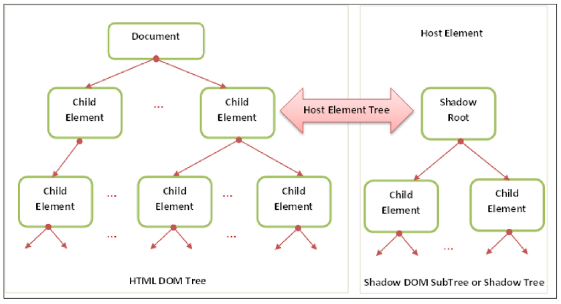
\includegraphics[width=\textwidth,height=\textheight,keepaspectratio]{shaDom.png}
			\caption{DOM und Shadow \ac{DOM} \cite[S. 22]{patel2015learning}}
			\label{img:shaDom}
		\end{figure}
		Die Folge dieser Kapselung ist, dass alles was dem \emph{Shadow tree} hinzugefügt wird, nur lokal Einfluss auf diesen hat. Die Gestaltung von Webelementen im \emph{Shadow root} wird dadurch vereinfacht.
		\ac{CSS} Selektoren können dadurch nicht von außerhalb des \emph{Shadow roots} auf diesen zugreifen und Selektoren, die innerhalb dieses definiert werden haben keinen Einfluss auf den normalen \ac{DOM}. Genauso verhält es sich mit dem Zugriff auf die \ac{DOM} Elemente des \emph{Shadow root}. Sie können nicht von außerhalb angesprochen werden, beispielsweise durch die Funktion \emph{document.querySelector()}, sondern können nur von Funktionen innerhalb des \emph{Shadow root} angesprochen werden.\cite[vgl.]{Bidelman2016}
		\begin{listing}
			\begin{JavaScriptcode*}{}
var header = document.createElement('header');
var shadowRoot = header.attachShadow({mode: 'open'});
var headline = document.createElement("h1");
var headlineText = document.createTextNode("headline");
headline.appendChild(headlineText);
shadowRoot.appendChild(headline);
			\end{JavaScriptcode*}
				\caption{JavaScript Code für das Erstellen eines Shadow DOM}
				\label{lst:javShaDom}
		\end{listing}
		In Listing \ref{lst:javShaDom} ist dargestellt, wie Mithilfe von JavaScript ein \emph{Shadow \ac{DOM}} erstellt wird. In Zeile zwei wird zuerst einem bestehendem Element ein \emph{Shadow root} hinzugefügt. Daraufhin wird eine Überschrift und deren Text erstellt und zusammengefügt. Zuletzt wird in Zeile sechs die Überschrift in den \emph{Shadow \ac{DOM}} eingefügt.
			\subsubsection{Slots}
			\emph{Shadow \ac{DOM}} kann auch mit anderen \ac{DOM} erweitert werden. Der Entwickler kann dem Nutzer seines \emph{Web Component} ermöglichen, diesen zu erweitern. Hierfür werden \emph{Slots} verwendet. 
			\begin{listing}
				\begin{HTMLcode*}{}
<ul id="contacts">
   <li>
      <slot name="title">Kein Titel</slot>
      <slot name="name">
         <p>Achtung<p>
         <h1>Kein Name<h1>
      </slot>
   </li>
</ul>
				\end{HTMLcode*}
				\caption{Nutzung von Slot Platzhalter-Elementen im Shadow DOM}
				\label{lst:sloNutShaDom}
			\end{listing}
			In Listing \ref{lst:sloNutShaDom} ist der \ac{HTML} Programmcode des \emph{Web Component} dargestellt, welcher im \emph{Shadow \ac{DOM}} später gerendert wird. Hier ist die Verwendung des \emph{Slot} Elements interessant. Dieses kann beim Einbinden des \emph{Web Component} später ausgestattet werden. Wird das Platzhalter-Element später nicht befüllt, wird das \emph{Fallback}, also die Ersatzfunktion, der Inhalt innerhalb des Elements, hier beispielsweise \enquote{Kein Titel} genutzt. Die Ersatzfunktion kann auch aus einem eigenen \ac{DOM} Baum bestehen, wie im \emph{Slot} \enquote{name} zu sehen ist.\cite[vgl.]{Bidelman2016} In Listing \ref{lst:sloNutLigDom} werden die, in Listing \ref{lst:sloNutShaDom} erstellten Platzhalter-Elemente, beim Verwenden des \emph{Web Component} in beispielsweise einer Webseite befüllt. Wie hier in Zeile fünf und sechs zu sehen ist, können einzelne Slots auch mit mehreren Elementen befüllt werden. Beim übersetzen des Programmcodes der Applikation werden alle Elemente, welche die passenden \emph{Slot} Attribute aufweisen in den \ac{DOM} übersetzt. Wenn im \emph{Shadow \ac{DOM}} ein \emph{Slot} Platzhalter ohne ein \enquote{name} Attribut definiert wird, werden alle vom Nutzer innerhalb des \emph{Web Components} erstellten Elemente in den \emph{DOM} geschrieben.
			\begin{listing}
				\begin{HTMLcode*}{}
<span slot="title">Dr.</span>
<span slot="title">Phil.</span>
<span slot="name">Michael</span>
				\end{HTMLcode*}
				\caption{Befüllen der Slot Elemente im DOM}
				\label{lst:sloNutLigDom}
			\end{listing}
			In Listing \ref{lst:renDom} ist der von den zwei vorhergehenden Listings kombinierte und gerenderte Inhalt zu sehen. Dies ist der \ac{DOM}, den man beispielsweise in einer Webseite sehen würde. Hier ist gut zu erkennen, wie die \emph{Slot} Elemente des \emph{Shadow \ac{DOM}} mit den später erstellten Elementen befüllt werden. Alle Elemente innerhalb des \emph{Web Component} mit dem Attribut \enquote{slot} werden in diesen übersetzt.
			\begin{listing}
				\begin{HTMLcode*}{}
<ul id="contacts">
   <li>
      <slot name="title">
	     <span>Dr.</span>
	     <span>Phil.</span>
	  </slot>
      <slot name="name">
	     <span>Michael</span>
      </slot>
   </li>
</ul>
				\end{HTMLcode*}
				\caption{Gerenderter DOM}
				\label{lst:renDom}
			\end{listing}
		
\chapter{Methodik dieser Arbeit}
\chapter{Adaptivität an den Nutzer}
Das Reaktion einer Internetseite, beziehungsweise von deren \emph{Web Components} die sich adaptiv an den Nutzer anpassen basiert auf drei Schritten. Als erstes werden Einstellungen und Vorlieben der Nutzer gesammelt und in einer für Maschinen verständlichen Form gespeichert. Der Ort an dem diese gespeichert werden, muss aus dem Netz erreichbar sein. Als nächstes müssen die Elemente der Internetseite darauf vorbereitet werden sich anzupassen. Dafür werden Funktionen und Ressourcen bereitgestellt, die sich bei Bedarf anpassen können. Nachdem dies erfolgt ist, kann die Internetseite, bei Aufruf durch einen bestimmten Nutzer eine Anforderung an den Speicherort stellen, die Informationen des bestimmten Nutzers zu übertragen. Daraufhin wird ein Befehl an die Elemente der Internetseite gestellt, die zu den jeweiligen Präferenzen und damit Nutzern, passenden Funktionen auszuführen. Dabei verändert sich das Aussehen und unter Umständen der Inhalt der Seite und beweist seine Adaptivität. \newline
Nachfolgend wird in dieser Arbeit darauf eingegangen in welcher Art sich an den Nutzer angepasst werden soll und wie diese Werte gespeichert und abgerufen werden. Als nächstes wird konfiguriert, wie sich die \emph{Web Components} an die entsprechenden Präferenzen anpassen werden und zuletzt wie das Ergebnis, adaptive Elemente von Webseiten, aussehen wird.
	\section{Präferenzen von Nutzern}
	Um eine Adaptivität zu ermöglichen, muss definiert werden, welche Bestandteile der Anwendung sich dynamisch verhalten, also an den Nutzer anpassen. Dazu mehr in Kapitel \ref{ref:konVonAda}. Vorher muss definiert werden, wie die Applikation insgesamt reagiert, also inwiefern sie ihren Zustand an den jeweiligen Nutzer anpasst. Hierfür werden alle Präferenzen eines Nutzers in einer Zusammenstellung gesammelt und notiert(\emph{Preference Set}).
	\section{Identifikation passender Preference Terms}
	Jeder Nutzer hat eigene Vorlieben und Einschränkungen beim Nutzen einer Anwendung. Somit unterscheidet sich die gesamte Nutzerschaft. Um diese abzubilden werden verschiedene Bezeichner definiert. Jeder Nutzer hat bei jedem dieser Bezeichner einen Wert. Somit wird ein Bezeichner-Wert Paar gebildet. Hier stellt sich die Frage, auf welcher Basis die Vorlieben und Einschränkungen definiert und organisiert werden.
		\subsection{WCAG Guidelines}
		Die \ac{WCAG 2.0} versuchen das Internet für alle Personen, unabhängig ihrer Einschränkung, zugänglicher zu machen. Hierfür schaffen sie Prinzipien und Richtlinien, auf Basis derer Internetseiten konzipiert werden können. Diese können sehr gut verwendet werden um herauszufinden, in welcher Art und Weise Anwendungen sich adaptiv an verschiedene Nutzer anpassen sollten.
			\subsubsection{Richtlinie 1.1 Text-Alternativen}
			Für Texte einer Anwendung sollen nicht aus Text bestehende Alternativen angeboten werden, beispielsweise große Druckbuchstaben, Brailleschrift, Sprache, Symbole oder einfachere Sprache. Parallel dazu sollen nicht textbasierte Inhalte auch durch eine textbasierte Alternative dargestellt werden können. 
			\subsubsection{Richtlinie 1.2 zeitbasierte Medien}
			Es sollen Alternativen für zeitbasierte Medien geschaffen werden.
			\subsubsection{Richtlinie 1.3 Anpassbar}
			Die Möglichkeit den Inhalt der Internetseite in verschiedenen Arten darzustellen, ohne Informationen oder Struktur zu verlieren, soll vorhanden sein sein.
			\subsubsection{Richtlinie 1.4 Unterscheidbar}
			Den Nutzern soll es erleichtert werden den Vordergrund vom Hintergrund zu unterscheiden. Dies soll bei visuellen und Audio-Elementen kongruent erfolgen. 
			\subsubsection{Richtlinie 2.1 Zugänglichkeit mit der Tastatur}
			Die gesamte Funktionalität der Anwendung sollte auch mit der Tastatur verwendet werden können.
			\subsubsection{Richtlinie 2.2 Ausreichend Zeit}
			Den Nutzern soll genügend Zeit zur Verfügung gestellt werden um den Inhalt zu lesen und nutzen.
			\subsubsection{Richtlinie 2.3 Anfälle}
			Der Inhalt sollte nicht in der Weise dargestellt werden, die bekannt dafür ist Anfälle auszulösen.
			\subsubsection{Richtlinie 2.4 Navigierbar}
			Es soll den Nutzern ermöglicht werden in der Anwendung zu navigieren, Inhalt zu finden und zu ermitteln an welcher Stelle sie sich befinden.
			\subsubsection{Richtlinie 3.1 Lesbarkeit}
			Der textbasierte Inhalt sollte lesbar und verständlich sein.
			\subsubsection{Richtlinie 3.2 Vorhersehbar}
			Internetseiten sollen in einer vorhersehbaren Art und Weise auftreten und funktionieren.
			\subsubsection{Richtlinie 3.3 Hilfestellung bei der Eingabe}
			Dem Nutzer soll geholfen werden, Fehler zu vermeiden und zu korrigieren.
			\subsubsection{Richtlinie 4.1 Kompatibel}
			Die Kompatibilität mit heutigen und zukünftigen Benutzeragenten und unterstützenden Technologien soll maximiert werden.			
			\cite[vgl.]{wcag}
		\subsection{Folgerung für Merkmale der Anwendung}
			\subsubsection{Kontrast}
			Um die \ac{WCAG 2.0} Richtlinie 1.4 zu erfüllen, sollte der Kontrast sich an den Nutzer anpassen. Der Bezeichner Kontrast definiert, ob und inwiefern der Nutzer einen Kontrastwert nutzen möchte, welcher vom Standard Kontrastwert abweicht. Beispielsweise erleichtert ein hoher Kontrast farbenblinden Nutzern Objekte vom Hintergrund zu unterscheiden. Für Nutzer ohne diese Einschränkung sind zu hohe Kontraste jedoch störend, da sie das Auge schnell ermüden.\cite[vgl S.234]{balzert2009webdesign}
			\subsubsection{Schrift}
			Die Wahl einer serifen oder grotesken, also serifenlosen Schriftart hat, wenn davon ausgegangen wird eine als allgemein lesbar bekannte Schriftart zu verwenden, keinen bestätigten Einfluss auf die Richtlinie 3.1, die Lesbarkeit eines Textes.\cite[vgl. S.157-161]{barrierefreiheit} Jedoch kann, um eine Adaptivität der Schriftart zu ermöglichen, dem Nutzer die Wahl gelassen werden, ob er eine serife oder groteske Schriftart nutzen möchte.
			Die Schriftgröße kann jedoch auch Einfluss auf die Richtlinie 3.1 nehmen. So kann eine zu große Schriftgröße, genauso wie eine zu kleine Schriftgröße die Lesbarkeit beeinträchtigen. Insbesondere älteren Menschen oder Nutzern mit Sehbeeinträchtigungen wird das Lesen eines Textes durch eine anpassbare Schriftart erleichtert.\cite[vgl. S.152]{barrierefreiheit} Somit ermöglicht ein Bezeichner Schriftgröße, zu welchem der Nutzer einen Wert wählen kann eine nützliche Adaptivität der Anwendung. 
			\subsubsection{Leserichtung}
			\label{ref:lesRic}
			Um die Richtlinie 3.1, die Lesbarkeit, zu erfüllen, sollte die Leserichtung sich an den Nutzer anpassen. Ohne diese Anpassung könnten Missverständnisse und Irritationen entstehen, da Texte von einer anderen Seite gelesen werden. So wird beispielsweise die arabische und hebräische von rechts oben nach links unten, die westliche von links oben nach rechts unten, geschrieben  \cite[vgl S.148]{emrich2013interkulturelles}
			
			\subsubsection{Anordnung der Elemente}
			Kongruent zum Kapitel \ref{ref:lesRic} ist zu bemerken, dass die Sprache des Nutzers und damit seine Leserichtung nicht nur einen Einfluss auf die Texte haben sollte, sondern insgesamt einen Einfluss auf die Gestaltung der Internetseite haben sollte. Aufgrund der Leserichtung fallen Elemente eines Internetauftritts an verschiedenen Stellen unterschiedlich auf. So ziehen bei einer Leserichtung von links nach rechts Elemente in der linken oberen Ecke eher die Aufmerksamkeit auf sich als Elemente in der rechten oberen Ecke, da diese erst danach gelesen werden. Im Gegensatz dazu fallen bei der Leserichtung von rechts nach links Elemente in der rechten oberen Seite schneller auf.\cite[vgl. S.47 f.]{meidl2013global}
			\begin{figure}
				\centering
				
\includegraphics[width=\textwidth,height=\textheight,keepaspectratio]{leserichtung.png}
				\caption{Einfluss der Leserichtung auf die Anordnung der Elemente\cite{elShaab}\cite{zeitOnline}}
				\label{img:lesRic}
			\end{figure}
			Ein Beispiel dazu bilden die deutsche und ägyptische Nachrichtenseite \enquote{Zeit Online} und \enquote{Al Shaab}, dargestellt in Abbildung  \ref{img:lesRic}. Hier ist im oberen Bereich die Kopfzeile der arabischsprachigen und darunter die Kopfzeile der deutschsprachigen Internetseite abgebildet. Hier sieht man ganz klar, wie im arabischsprachigen Bereich die Elemente eher nach rechts ausgerichtet sind und wichtige Elemente, wie beispielsweise der Name der Zeitung ganz rechts oben angeordnet sind. Im deutschsprachigem Internetauftritt sind die Elemente nach links ausgerichtet und der Name der Webseite ist weit oben links.
			\subsubsection{Text-Alternativen}
			Die Richtlinie 1.1 definiert, dass zu jedem Text eine Alternative geboten wird. Darüber hinaus sollen die nicht textbasierten Inhalte nach Bedarf durch einen Text dargestellt werden können. Dem Nutzer sollte ermöglicht werden in seinen Präferenzen anzugeben, ob er den Text, oder dessen Alternativen angezeigt bekommen möchte.
			\subsubsection{Geschwindigkeit}
			Die Richtlinie 2.2 sichert dem Nutzer ausreichend Zeit zu, den Inhalt zu lesen und zu nutzen. Dies sollte adaptiv an den Nutzer angepasst werden, da manchen Nutzer mehr oder weniger Zeit für eine bestimmte Aufgabe benötigen. Beispielsweise werden bestimmte Navigationselemente durch ein Verweilen der Maus auf diesen ausgeklappt. Sobald die Maus nicht mehr auf dem Element verweilt wird es wieder eingeklappt. Hier sollte es dem Nutzer ermöglicht werden die Zeitspanne anzupassen bevor das Element wieder einklappt, da es ihm andernfalls nicht möglich sein könnte das Element schnell genug zu nutzen.
		
			
		\subsection{Speichern der Nutzer Präferenzen}
		Die Präferenzen der verschiedenen Nutzer, also die Bezeichner-Wert Paare müssen gespeichert werden. Der Speicherort muss an das Netz angeschlossen sein, da die Werte zur Laufzeit der Anwendung, beziehungsweise beim Laden der Internetseite abgerufen werden müssen.
		
		\subsection{Herunterladen der Nutzer Präferenzen}
		Um die Präferenzen der Nutzer zu verwenden und auf Basis dieser die Webseite anzupassen, muss eine Möglichkeit geschaffen werden, die Zusammenstellung der Präferenzen beim Aufruf der Anwendung abzufragen. Hierfür wird ein \emph{REST-Client} verwendet. Dieser sendet beim Aufruf der Anwendung einen Befehl an einen bestimmten, an das Netz angeschlossenen, Ort. Dabei wird diesem Ort mitgeteilt, für welche Person die Zusammenstellung angefragt wird. Daraufhin erhält die Anwendung als Antwort alle Präferenzen der mitgeteilten Person und kann auf Basis dieser die Anwendung anpassen.
			\subsubsection{Was bedeutet REST}
			\emph{\ac{REST}} ist ein Protokoll um Daten in einer verteilten Umgebung auszutauschen. Es basiert auf den folgenden Prinzipien.
			\begin{description}  
				\item  [Adressierbarkeit von Ressourcen]
				Jede Ressource sollte von einem einzigartigen Bezeichner identifiziert werden können.
				
				\item [Einfache und einheitliche Schnittstelle]
				Das \ac{REST} Protokoll basiert auf dem \ac{HTML} Protokoll. Es werden die von der \ac{HTTP}-Technologie bekannten Methoden verwendet. Dies macht \ac{REST} Protokoll 
				simpel und einheitlich.
				
				\item  [Repräsentation] 
				Die Ressourcen können in verschiedenen Formen repräsentiert werden. Bei Änderung oder Anfrage der Ressource wird immer eine Repräsentation genutzt. Somit kann in einer Anfrage definiert werden, in welcher Form der Repräsentation die Antwort erfolgen soll.
				
				\item [Zustandslos]
				Es werden keine Zustände auf dem \emph{Server} gespeichert. Zustandsinformationen werden vom \emph{Client} gehandhabt und bei Bedarf an den Server gesendet.
				
				\item [Cashing möglich]
				Der \emph{Client} sollte die Möglichkeit haben,  die Antworten für späteren Gebrauch zu speichern.	\cite[vgl. S.77]{chauhan2014asp} 
			\end{description}
		\subsubsection{Der Client}
		Die Funktion um die Präferenzen eines bestimmten Nutzers abzufragen basiert auf der \emph{jQuery.ajax()} Funktion. Dies ist eine Funktion des \emph{jQuery Frameworks} , welche eine asynchrone Anfrage an einen Ort stellt, basierend auf dem \ac{HTTP} Protokoll.\cite[vgl.]{jquAja}
		\begin{listing}
			\begin{JavaScriptcode*}{}
function restCall (url){
   jQuery.ajax({
      //URL setzen, um Wert von bestimmtem Nutzer anzufragen
      url: url,
      data: {
         format: 'json'
      },
      error: function(request, status, error) {
         //Fehlermeldung ausgeben
      },
      dataType: 'json',
      success: function(data) {
         //Speichern der empfangenen Beispieldaten
         var reading_direction = data.reading_direction;
         var contrast = data.contrast;
         //Seite entsprechend der empfangenen Präferenzen ändern
         update(reading_direction, contrast);
      },
      type: 'GET'
   });
}
			\end{JavaScriptcode*}
			\caption{Programmcode zum Abfragen der Nutzerpräferenzen}
			\label{lst:jquAja}
		\end{listing}
		Wie in Listing \ref{lst:jquAja} dargestellt führt die Funktion \enquote{restCall} eine asynchrone Anfrage aus. Sie erwartet ein Argument \enquote{url}. Dieses Argument wird gesetzt um einen entsprechenden Speicherort der Zusammenstellung der Präferenzen und den gewünschten Nutzer anzufragen. Ein Beispiel dieses Speicherorts könnte \enquote{http://www.speicherort.de/praeferenzen/nutzer1} sein. In Zeile fünf und sechs wird das Datenformat der erwarteten Antwort definiert, hier wird das Format \ac{JSON} genutzt. Ab Zeile acht wird die Fehlerbehandlung definiert, hier wird gewählt, was bei einem Fehler, beispielsweise einem nicht Erreichen des Speicherorts, passiert. Bei erfolgter Antwort des Speicherorts wird die \enquote{succes} Funktion aufgerufen. Hier werden die empfangenen Daten zuerst gespeichert, um sie dann in der \enquote{update} Funktion nutzen. Diese passt das \emph{Web Component} adaptiv, entsprechend der Präferenzen des Nutzers an. In Zeile 19 wird definiert, welche Art eines \ac{REST} Aufrufs erfolgen soll. Hier wird ein \emph{GET} Aufruf genutzt, da Daten vom Speicherort abgerufen werden sollen.
\chapter{Adaptivität von bestehenden Web Components}
	In den folgenden Kapiteln werden bestehende \emph{Web Components} ausgewählt, untersucht und um eine Adaptivität zu ermöglichen, angepasst. Hierfür werden Elemente aus dem Katalog der Internetseite \enquote{customelements.io} gewählt.\cite{cusEleIo}
	\section{Die Elemente}
	Die erste Auswahl ist das Element \enquote{google-map}. Es ist ein \emph{Web Component}, der die Anzeige einer \emph{Google Map}, also einer Karte, ermöglicht. Diese Karte kann personalisiert und durch Wegbeschreibungen oder Markierungen ergänzt werden.\cite{gooMap}
	
	\section{Anpassung dieser Web Components}
		\subsection{google-map}
			\subsubsection{Konzeption zur Adaptivität}
			\label{ref:konVonAda}
			Abbildung \ref{img:gmap} zeigt die Ansicht einer \enquote{Google Map}, im weiteren Karte genannt. Sie nutzt einerseits farbige Abbildungen und Symbole, andererseits auch verschiedene Texte. Um eine Adaptivität zu ermöglichen, sollte Einfluss auf den Kontrast, die Schrift, die Leserichtung und damit die Anordnung der Elemente und Text-Alternativen genommen werden. Der Kontrast der Kartenelemente sollte sich adaptiv an den Nutzer anpassen. Hier sollten die Straßen, Gebäude, Grünflächen und ähnliche Elemente, welche durch Farbunterschiede dargestellt werden, sich stark voneinander abheben können, um allen Nutzern das Lesen der Karte zu ermöglichen. Des weiteren sollte sich die Schrift, also die Bezeichner der Kartenelemente, wie Städte, Straßen oder besondere Gebäude anpassen. Auch sollte sich die Schrift auf den Buttons und in der Suchleiste angleichen. Hier sollte es dem Nutzer ermöglicht werden zwischen einer kleinen oder großen und einer serifen oder grotesken Schriftart zu wählen. Um sich an die Leserichtung des Anwenders anzupassen muss zum einen der Text angepasst werden und zum anderen der Aufbau des \emph{Web Components} sich verändern. So sollten das wichtigste Element, die Suchleiste inklusive der Einstellungen, bei einer Leserichtung von links nach rechts in der linken oberen Ecke befinden und bei einer Leserichtung von rechts nach links in der rechten oben Ecke befinden. Dementsprechend würden sich der derzeitige Aufbau der Karte bei einer Leserichtung von rechts nach links spiegeln. Zuletzt sollten für die Texte Text-Alternativen geboten werden und Bestandteile der Karte welche eine Funktion erfüllen und nur durch Bilder oder Symbole dargestellt werden, auch als Text angeboten werden. 
			\begin{figure}
				\centering
				
\includegraphics[width=\textwidth,height=\textheight,keepaspectratio]{gmap.png}
				\caption{Google Map Ansicht\cite{gooMapOri}}
				\label{img:gmap}
			\end{figure}
			\subsubsection{Umsetzung Programmierung}
			Zuerst wird die Anpassung Kontrastwert vorgenommen. Hier sollte zu Beginn auf die Erstellung einer \enquote{Google Map} genauer eingegangen werden.
		\subsection{Web Component Zwei}
		\subsection{Web Component Drei}
\chapter{Vergleich}
	\section{Vergleich mit Polymer}
	

	\printbibliography
\end{document}